\input{../lib.tex}
\doctitle{Filtre}

\section{Filtre\\}

\subsection{Introduction}
Le MLI a besoin d'un signal sinusoïdal pour fonctionner, cependant, le VCO fournit un signal triangulaire. Il est donc nécessaire d'avoir un filtre intermédiaire permettant de transformer le signal du VCO en signal sinusoïdal ou tout du moins pseudo-sinusoïdal.\\
\begin{figure}[h]
\centering
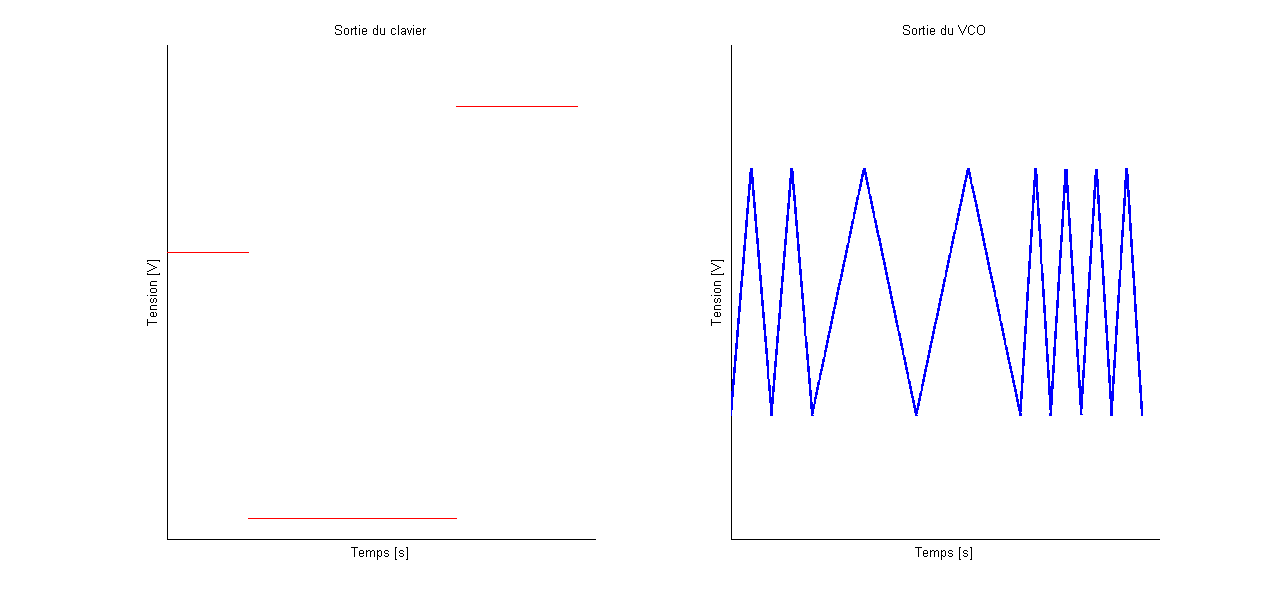
\includegraphics[scale=0.3]{in-out.png}
\caption{Entrée et sortie du filtre: objectif}
\end{figure}\\
\subsection{Fonctionnement}
\begin{figure}[h]
\centering
\includegraphics[scale=0.3]{circuitcolored.png}
\caption{Filtre}
\end{figure}
Le filtre utilise les diodes pour faire varier le circuit en fonction de la tension de sortie . Le circuit possède ainsi 4 états différents selon la tension de sortie:
\begin{enumerate}
\item Elle est trop basse pour traverser la moindre diode.\\
Dans ce cas-ci, seule la partie bleue du circuit est active, il n'y a pas de courant, la tension d'entrée est don égale à la tension de sortie.
\item Elle est suffisante pour traverse une diode.\\
Ici, la partie rouge est active aussi. On se retrouve donc avec un diviseur de tension qui diminuera la  tension de sortie par rapport à la valeur d'entrée.
\item Elle est suffisante pour traverser deux diodes.\\
La partie orange s'active en plus, ce qui mettra en parallèle les resistances R1 et R2, ce qui réduira encore d'avantage la tension de sortie.
\item Elle est suffisante pour être écrêter par trois diodes.\\
À partir d'ici, la resistance interne\footnote{À noter que si les diodes étaient idéales, le circuit fonctionnerait moins bien: au lieu d'obtenir un sommet de courbe de tension arrondi dû à la résistance dynamique variante des diodes, on aurait un sommet de courbe horizontal à cause du lien direct à la masse. On pourrait cependant rajouter une résistance R3 très faible derière les diodes pour redresser légèrement le sommet de la courbe.} des 3 diodes jaunes va se mettre en parallèle avec R1 et R2. Étant donné que la resistance interne des diodes est très faible comparée à R0, il n'y a que peu de tension qui s'ajoutera encore à la tension de sortie.
\end{enumerate}
\subsection{Détails du circuit}
\begin{enumerate}
\item Signal d'entrée\\
Le signal d'entrée doit être suffisament grand pour commencer à être écrêter par trois diodes en série, le signal de sortie cilminera donc aux alentours de 1.9V. Le signal d'entrée est donc le signal triangulaire circonscrit au signal sinusoïdal d'amplitude 1.9V, soit un signal triangulaire d'amplitude 3V.
\item Valeur des résistances\\
\begin{enumerate}
\item première approximation\\
R0 a été définie à 1k\\
R1 vaut 7.9k afin que la pente de la tension avec le diviseur R0/R1 soit égale à la pente moyenne de y=1.9*sin(C*x) entre y=0.6 et y=1.2 (soit 0.87*C)\\
R2 vaut 2.2k afin que la pente de la tension avec le diviseur R0/(R1//R2) soit égale à la pente moyenne de y=1.9*sin(C*x) entre y=1.2 et y=1.8 (soit 0.58*C)\\
Avec cette première approximation, le taux de distortion harmonique total compris entre 0.51\% (500Hz) et 0.5\%(10kHz).
\item seconde approximation\\
Pour améliorer ensuite le pseudo-sinus, des tests empiriques ont amené à une valeur de 12.1k pour R1 et de 2.1k pour R2.\\
Avec ces nouvelles valeurs, le taux de distortion harmonique total compris entre 0.3\% (500Hz) et 0.23\% (10kHz).
\end{enumerate}

\end{enumerate}
\input{../footer.tex}
\begin{figure}[h]
\centering
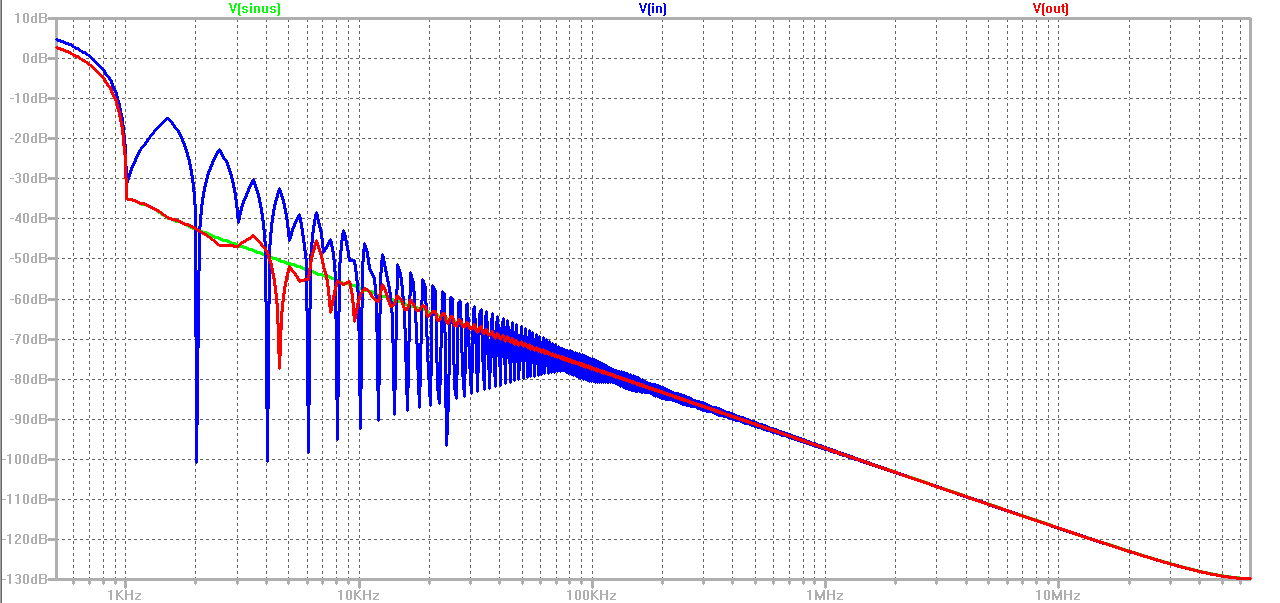
\includegraphics[scale=0.3]{FFT.png}
\caption{FFT avec les résistances de la seconde estimation.}
\end{figure}
\subsection{Confontation théorie/pratique}
\begin{figure}[h]
\centering
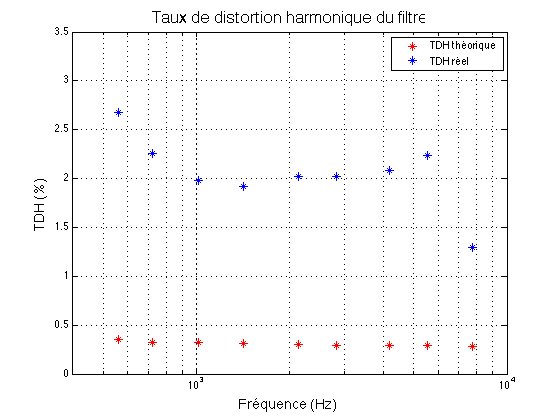
\includegraphics[scale=0.3]{THD.png}
\caption{Confrontation THD réel et théorique}
\end{figure}
Dans la pratique, l'on peut remarquer que le THD\footnote{Pour "Total Harmonic Distortion" ou taux de distortion harmonique total.} est non seulement beaucoup plus important que dans la réalité, mais aussi beaucoup plus variable. Cela est principalement dû au manque de précision des composants dans le filtre et en amont\footnote{En effet, cela cause une imprécision dans le signal d'entrée du filtre qui n'est pas exactement un signal triangulaire +3V/-3V}. Mais c'est aussi dû aux glitchs provoqués par le sigma-delta qui perturbent le pseudo-sinus.
\subsection{Améliorations possibles}
\begin{enumerate}
\item Coder un programme capable de calculer avec précision R0, R1, R2 et la tension d'entrée afin de réduire au maximum le taux de distortion harmonique.
\item S'arranger pour que les données pratiques soient plus proches des données théoriques afin de minimiser l'erreur dûe à la tolérance des composants.
\end{enumerate}

\end{document}
